\documentclass{FastFyp}
\usepackage{tikz}
\usetikzlibrary{arrows.meta}
\definecolor{wnavy}{HTML}{1F4E79}
\definecolor{wblue}{HTML}{2E75B6}
\definecolor{worange}{HTML}{C55A11}
\definecolor{wtint}{HTML}{EAF1F8}

\begin{document}
\newcommand{\university}{National University of Computer and Emerging Sciences, Lahore}
\newcommand{\fyptitle}{WAF Studio: An Explainable Reverse-Proxy Web Application Firewall}
\newcommand{\Studentone}{M. Wahaj}
\newcommand{\Studenttwo}{Shazil Hamzah}
\newcommand{\Studentthree}{Muhammad Saad}
\newcommand{\Studentfour}{Nufil Anwar}
\date{\today}
\renewcommand{\contentsname}{Table of Contents}

\makeatletter
    \begin{titlepage}
        \includegraphics[width=0.2\linewidth]{Figures/nulogo.png}\hfill
        \includegraphics[width=0.2\linewidth]{Figures/fast.png}\\
        \begin{center}
            {\large\bfseries \university}\\[7ex]
            \includegraphics[width=0.4\linewidth]{Figures/fastlogo.png}\\[8ex]
            {\huge \bfseries \fyptitle }\\[10ex]
            {\Studentone}\\{\Studenttwo}\\{\Studentthree}\\{\Studentfour}\\[14ex]
            {Information Security Project Documentation}\\
            {\large \@date}
        \end{center}
    \end{titlepage}
\makeatother
\frontmatter

\pagestyle{empty}
\section*{Abstract}
WAF Studio is a learning web application firewall that runs as a reverse proxy in front of a deliberately vulnerable test shop. It parses and normalizes each request, matches it against a validated rule language, scores the result, and either forwards or blocks the request while recording the evidence that explains the decision. A role-based browser console supports analysis, tuning with scoped exceptions, reporting and a tamper-evident audit log. In a controlled evaluation the system passed 117 of 123 mandatory checks, raised no false positives on 68 benign inputs, and added under 2 ms at the 95th percentile.

\section*{Executive Summary}
Most firewall demonstrations show only that a request was blocked. WAF Studio was built so that a learner can also see \emph{why}: which rules matched, where in the request they matched, what decoding was needed, and how the points added up to a decision.

The system has four parts: an inspecting reverse proxy on port 8080, a security engine shared with the console, a role-based web console on port 3000 backed by SQLite, and a vulnerable test shop on port 3001. Everything listens on 127.0.0.1 and uses fake data. The engine ships with 41 rules, flags a request at a score of 3 and blocks it at 5, and supports a monitor mode that only logs. Administrators tune the system through versioned rules and configuration, and operators request scoped exceptions that a different administrator must approve.

The final acceptance run passed 782 of 782 automated tests with no known vulnerabilities in the production dependencies. The evaluation passed 117 of 123 mandatory checks; the six failures are evasion attempts (split or encoded payloads) that are reported rather than hidden. On a controlled corpus of 80 attacks and 68 benign requests the engine reached 95\% recall and 100\% precision. The results come from a synthetic corpus on one laptop and are not a claim about internet traffic.

\pagestyle{fancy}
\pagebreak
\tableofcontents

\pagebreak
\listoffigures
\addcontentsline{toc}{chapter}{List of Figures}
\pagebreak
\listoftables
\addcontentsline{toc}{chapter}{List of Tables}

\mainmatter

%==================================================================
\chapter{Introduction}
This chapter states the purpose of the document, the objectives and scope of the project, and the terms used in the rest of the report.

\section{Purpose of this Document}
This document describes the design, implementation and evaluation of WAF Studio, the Information Security project of Class 3, Group 12 (Proposal 44). It is a short technical reference for readers who need to run, understand or extend the system. Longer material such as the requirements, the STRIDE threat model and the per-input evaluation results is kept in the project's \texttt{docs} folder and is summarized here rather than repeated.

\section{Objectives}
The proposal asks for a functioning system, not a design mock-up. WAF Studio therefore aims to (i) accept controlled input from both a real HTTP proxy and a console, (ii) make an explainable security decision for every request, (iii) retain reproducible evidence of each decision, and (iv) protect its own users and data. The same engine and active policy serve both entry points, so a request analysed in the console receives the decision it would receive through the proxy.

\section{Scope}
The seven required modules are request parsing, a rule language, scoring, block and monitor modes, rate limits, an audit console, and tuning with exceptions. All seven are implemented (Table~\ref{tab:modules}). Production hosting, paid services, native mobile applications, external targets and real attack deployment are out of scope. The test shop contains fake users, products and files, and its vulnerabilities are confined to an in-memory database and a sandboxed folder.

\begin{table}[!h]
\centering
\caption{The seven required modules and where each one lives (paths are under \texttt{src/} unless noted).}
{\small\singlespacing\renewcommand{\arraystretch}{1.3}
\begin{tabular}{|p{4.0cm}|p{9.5cm}|}
\hline
\textbf{Module} & \textbf{Implementation} \\
\hline
Request parsing & \texttt{engine/parser.js}, \texttt{engine/normalize.js} \\
\hline
Rule language & \texttt{engine/dsl.js}, \texttt{engine/regexguard.js}, \texttt{engine/evaluate.js} \\
\hline
Scoring & \texttt{engine/scoring.js}, \texttt{engine/explain.js} \\
\hline
Block and monitor modes & \texttt{engine/modes.js} \\
\hline
Rate limits & \texttt{engine/ratelimit.js}, \texttt{auth/rateLimit.js} \\
\hline
Audit console & \texttt{public/} (console), \texttt{api/routes/audit.js}, \texttt{db/repositories/audit.js} \\
\hline
Tuning and exceptions & \texttt{engine/exceptions.js}, \texttt{api/routes/exceptions.js} \\
\hline
\end{tabular}}
\label{tab:modules}
\end{table}

\section{Definitions, Acronyms, and Abbreviations}
\textbf{WAF}: Web Application Firewall\\
\textbf{DSL}: Domain-Specific Language (the rule language)\\
\textbf{CSP}: Content Security Policy\\
\textbf{CSRF}: Cross-Site Request Forgery\\
\textbf{STRIDE}: a threat-classification scheme used for the threat model\\
\textbf{p95}: the 95th percentile of a measurement\\
\textbf{TP, FP, TN, FN}: true positives, false positives, true negatives and false negatives

\section{Report Outline}
Chapter~2 describes the architecture and how to run the system. Chapter~3 explains the security engine. Chapter~4 covers the console and the security of the application itself. Chapter~5 presents the evaluation, and Chapter~6 states the limitations and conclusions.

%==================================================================
\chapter{System Overview and Design}
\section{Architecture}
Figure~\ref{fig:arch} shows the two ways a request reaches the engine. A browser user signs in to the console, which calls the API. Any HTTP client can instead send traffic to the reverse proxy. Both paths call the same security engine with the same active policy, and events, policy versions and the audit chain are stored in SQLite. Allowed requests are forwarded to the test shop.

\begin{figure}[!h]
\centering
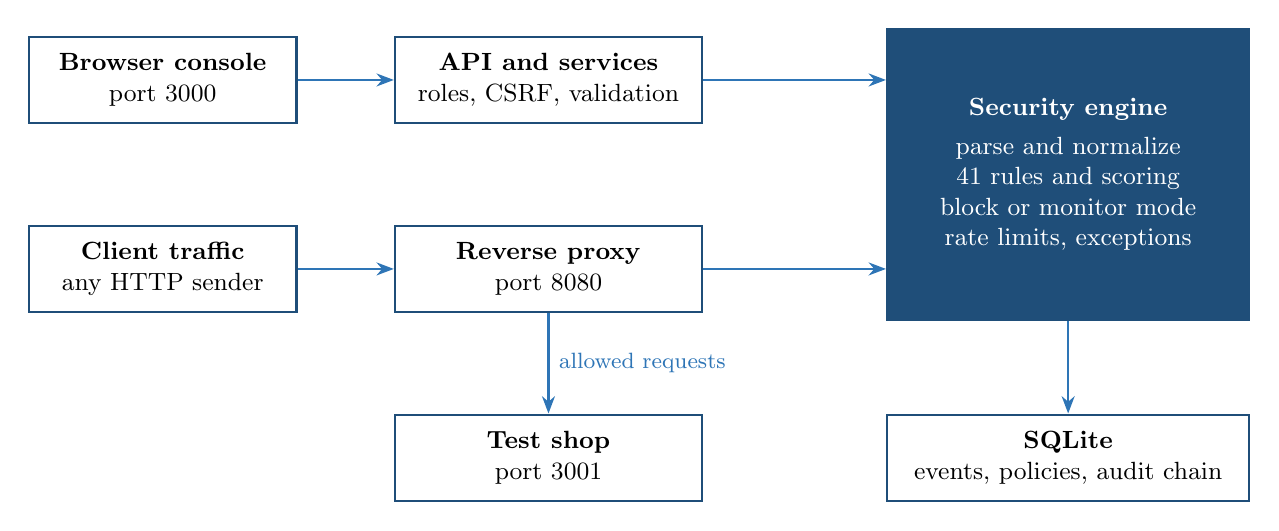
\begin{tikzpicture}[font=\small, >={Stealth[length=2.2mm]},
  box/.style={draw=wnavy, thick, fill=white, align=center, minimum height=1.1cm, text=black},
  big/.style={draw=wnavy, thick, fill=wnavy, align=center, text=white}]
  \node[box, minimum width=3.4cm] (br) at (1.7,3.4) {\textbf{Browser console}\\port 3000};
  \node[box, minimum width=3.9cm] (api) at (6.6,3.4) {\textbf{API and services}\\roles, CSRF, validation};
  \node[box, minimum width=3.4cm] (cl) at (1.7,1.0) {\textbf{Client traffic}\\any HTTP sender};
  \node[box, minimum width=3.9cm] (px) at (6.6,1.0) {\textbf{Reverse proxy}\\port 8080};
  \node[big, minimum width=4.6cm, minimum height=3.7cm] (en) at (13.2,2.2) {\textbf{Security engine}\\[1mm]parse and normalize\\41 rules and scoring\\block or monitor mode\\rate limits, exceptions};
  \node[box, minimum width=3.9cm] (sh) at (6.6,-1.4) {\textbf{Test shop}\\port 3001};
  \node[box, minimum width=4.6cm] (db) at (13.2,-1.4) {\textbf{SQLite}\\events, policies, audit chain};
  \draw[->, thick, wblue] (br) -- (api);
  \draw[->, thick, wblue] (api.east) -- (en.west |- api.east);
  \draw[->, thick, wblue] (cl) -- (px);
  \draw[->, thick, wblue] (px.east) -- (en.west |- px.east);
  \draw[->, thick, wblue] (px) -- node[right, font=\footnotesize] {allowed requests} (sh);
  \draw[->, thick, wblue] (en) -- (db);
\end{tikzpicture}
\caption{The proxy path and the console path share one security engine and one database.}
\label{fig:arch}
\end{figure}

If the shop is unreachable the proxy returns a safe 502, and if inspection itself fails unexpectedly the request fails closed with a 503. The proxy block page shows an event identifier but not the detailed rule that fired.

\section{Components}
Table~\ref{tab:folders} lists the main folders of the repository and what each one is responsible for.

\begin{table}[!h]
\centering
\caption{Main folders of the repository and their responsibilities.}
{\small\singlespacing\renewcommand{\arraystretch}{1.3}
\begin{tabular}{|p{4.9cm}|p{8.6cm}|}
\hline
\textbf{Folder} & \textbf{Responsibility} \\
\hline
\texttt{src/engine} & Parsing, normalization, rule language, scoring, modes, rate limit, exceptions, explanation (no database or network access) \\
\hline
\texttt{src/rules} & The 41 default rules \\
\hline
\texttt{src/proxy} & Reverse proxy and block pages \\
\hline
\texttt{src/api} & JSON API for the console, validation and error handling \\
\hline
\texttt{src/auth} & Password hashing, sessions, login throttling, role checks \\
\hline
\texttt{src/db} & SQLite schema and repositories, append-only audit chain \\
\hline
\texttt{src/services} & Analysis, audit writing, first-run seeding, logging, client pseudonyms \\
\hline
\texttt{src/reports} & Sanitized JSON, CSV and HTML export \\
\hline
\texttt{public} & Browser console (plain JavaScript modules) \\
\hline
\texttt{target} & Deliberately vulnerable test shop with fake data \\
\hline
\texttt{fixtures}, \texttt{test}, \texttt{scripts} & Synthetic inputs, 782 tests, setup and evaluation tools \\
\hline
\end{tabular}}
\label{tab:folders}
\end{table}

\section{Technology}
WAF Studio runs on Node.js 22.13 or newer. The only production dependencies are Express 4.22.3 and http-proxy 1.18.1; storage uses the SQLite module built into Node. The console is written as plain JavaScript modules with no framework and loads nothing from the network, which lets the server send a strict Content Security Policy.

\section{Roles and Access}
Three roles are enforced on the server, and the interface only hides what a role cannot use (Table~\ref{tab:roles}).

\begin{table}[!h]
\centering
\caption{What each role can do.}
{\small\singlespacing\renewcommand{\arraystretch}{1.3}
\begin{tabular}{|p{2.4cm}|p{11.1cm}|}
\hline
\textbf{Role} & \textbf{Main capabilities} \\
\hline
Viewer & Overview, event list with sanitized summaries, own account \\
\hline
Operator & Viewer rights plus evidence detail, comparison, replay, request analysis, sample import, reading rules and configuration, requesting exceptions, exporting reports \\
\hline
Administrator & Operator rights plus editing rules and configuration, approving or rejecting exceptions, the audit log and user management \\
\hline
\end{tabular}}
\label{tab:roles}
\end{table}

\section{Installation and Use}
Setup creates the database, the default rules and four accounts (admin, admin2, operator, viewer) and prints their passwords once.
{\small\singlespacing
\begin{verbatim}
npm ci          npm run setup          npm start
\end{verbatim}}
The console is then at \texttt{http://127.0.0.1:3000}, the protected proxy at port 8080 and the test shop at port 3001. Running \texttt{npm test} executes the full suite, and \texttt{npm run evaluate} reproduces the evaluation.

%==================================================================
\chapter{Security Engine}
\section{Parsing and Normalization}
The parser validates the method, URL, header and argument counts and the body size, then extracts values from the query, JSON, form, multipart and cookie data. Defaults are a 4,096-character URL, 100 headers, 200 arguments, three decoding rounds, a 64~KiB inspection window and a 1~MiB maximum body; larger bodies are rejected with status 413. A body between 64~KiB and 1~MiB is forwarded with only its prefix inspected and an explicit anomaly recorded.

Each value is kept in several normalized forms so that disguised payloads still match: repeated URL decoding, \%u escapes, HTML entities, Unicode NFKC, removal of null and invisible characters, SQL comment handling, and case, whitespace and path normalization. The transformation that was needed is stored as evidence, so an encoded match can be explained.

\section{Rule Language}
Rules are written in a small documented language. Invalid syntax is rejected with a line and column, and regular expressions that could backtrack catastrophically are refused by a conservative guard. Every stored rule has a version.

{\small\singlespacing
\begin{verbatim}
rule 942100 "SQLi boolean tautology" {
  when args matches /\b(or|and)\b\s+['"]?\d+['"]?\s*=\s*['"]?\d+/i
  severity critical
  score 5
  category sqli
  tags sqli, owasp-a03
  description "Tautology used to bypass WHERE clauses"
}
\end{verbatim}}

\section{Scoring and Modes}
Each matching rule contributes its points once per request, together with the matched location, excerpt and decoding steps. Anomaly points, for example from malformed input, are added to the same total. The default thresholds are 3 to flag and 5 to block (Figure~\ref{fig:pipeline}). In block mode a blocked request receives a 403 response; in monitor mode the request is forwarded and the event records that it would have been blocked.

\begin{figure}[!h]
\centering
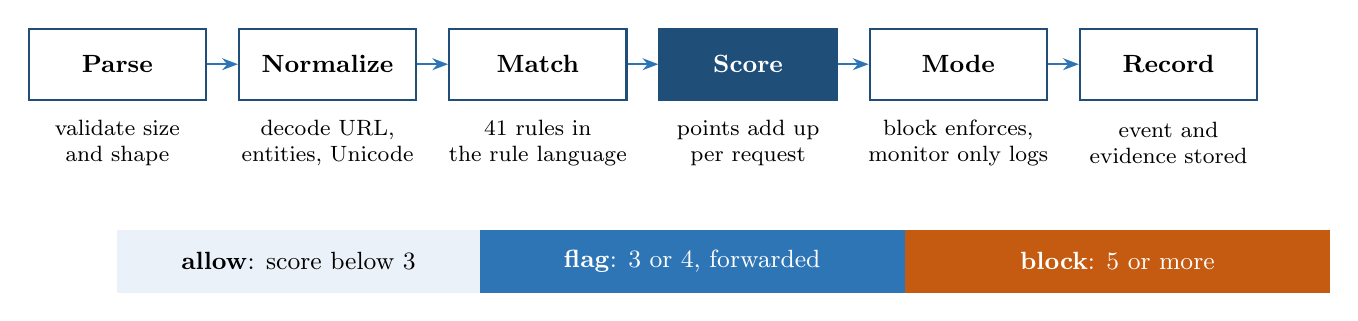
\begin{tikzpicture}[font=\small, >={Stealth[length=2mm]},
  st/.style={draw=wnavy, thick, fill=white, minimum width=2.25cm, minimum height=0.9cm, align=center}]
  \foreach \i/\t/\d in {0/Parse/{validate size\\and shape},1/Normalize/{decode URL,\\entities, Unicode},2/Match/{41 rules in\\the rule language},3/Score/{points add up\\per request},4/Mode/{block enforces,\\monitor only logs},5/Record/{event and\\evidence stored}} {
    \pgfmathsetmacro{\x}{\i*2.67}
    \ifnum\i=3 \node[st, fill=wnavy, text=white] (n\i) at (\x,0) {\textbf{\t}};
    \else \node[st] (n\i) at (\x,0) {\textbf{\t}}; \fi
    \node[font=\footnotesize, align=center] at (\x,-1.0) {\d};
  }
  \foreach \i/\j in {0/1,1/2,2/3,3/4,4/5} \draw[->, thick, wblue] (n\i) -- (n\j);
  \node[minimum width=4.6cm, minimum height=0.8cm, fill=wtint, align=center, draw=none] (a) at (2.3,-2.5) {\textbf{allow}: score below 3};
  \node[minimum width=5.4cm, minimum height=0.8cm, fill=wblue, text=white, align=center] (b) at (7.3,-2.5) {\textbf{flag}: 3 or 4, forwarded};
  \node[minimum width=5.4cm, minimum height=0.8cm, fill=worange, text=white, align=center] (c) at (12.7,-2.5) {\textbf{block}: 5 or more};
\end{tikzpicture}
\caption{Each request passes through six steps, and the total score selects the outcome.}
\label{fig:pipeline}
\end{figure}

\section{Rate Limits and Exceptions}
The proxy uses a sliding window of 300 requests per 60 seconds for each client pseudonym. Console logins have separate per-account and per-client throttles, and repeated analysis from the console is also limited.

When a rule produces a false positive, an operator can preview the impact and request an exception scoped to a path prefix, a method and a location. A different administrator must review it; an operator cannot approve it. Approved exceptions suppress one rule within that narrow scope and are recorded as evidence in every decision they affect. Replaying an event creates a new event and keeps the original, and revoking an exception restores the original enforcement. High-impact configuration changes require a confirmation and a written reason.

\section{Default Rule Set}
The 41 default rules are grouped by category (Table~\ref{tab:rules}). Scores are calibrated so that a score of 5 is a strong indicator that blocks alone, 3 or 4 is suspicious and flags alone, and 1 or 2 is weak context that never blocks alone. Patterns use bounded repetition so that they stay linear on large bodies.

\begin{table}[!h]
\centering
\caption{Default rules by category.}
{\small\singlespacing\renewcommand{\arraystretch}{1.3}
\begin{tabular}{|p{4.6cm}|p{2.8cm}|p{1.8cm}|}
\hline
\textbf{Category} & \textbf{Rule ids} & \textbf{Rules} \\
\hline
Scanner signatures & 913xxx & 5 \\
\hline
Protocol violations & 920xxx & 6 \\
\hline
Path traversal & 930xxx & 5 \\
\hline
Command injection & 932xxx & 5 \\
\hline
Cross-site scripting & 941xxx & 10 \\
\hline
SQL injection & 942xxx & 10 \\
\hline
\textbf{Total} & & \textbf{41} \\
\hline
\end{tabular}}
\label{tab:rules}
\end{table}

%==================================================================
\chapter{Console and Application Security}
\section{Web Console}
The console groups its screens by task: \emph{Activity} (Overview, Events with inline report export), \emph{Tools} (Analyze, combining single-request inspection and batch JSON import), \emph{Policy} (Rules, Configuration, Exceptions) and \emph{Administration} (Audit log, Users), plus an account page in the header. Each role sees only the groups it can use, and secondary forms (such as creating rules, exception requests and users, or viewing version history) expand on demand to keep the interface minimal. The Overview (Figure~\ref{fig:dash}) answers the most common question first: how many requests were inspected, blocked and passed in a chosen time range, with a recommended next action, an hourly activity chart and the most frequent detection categories.

\begin{figure}[!h]
\centering
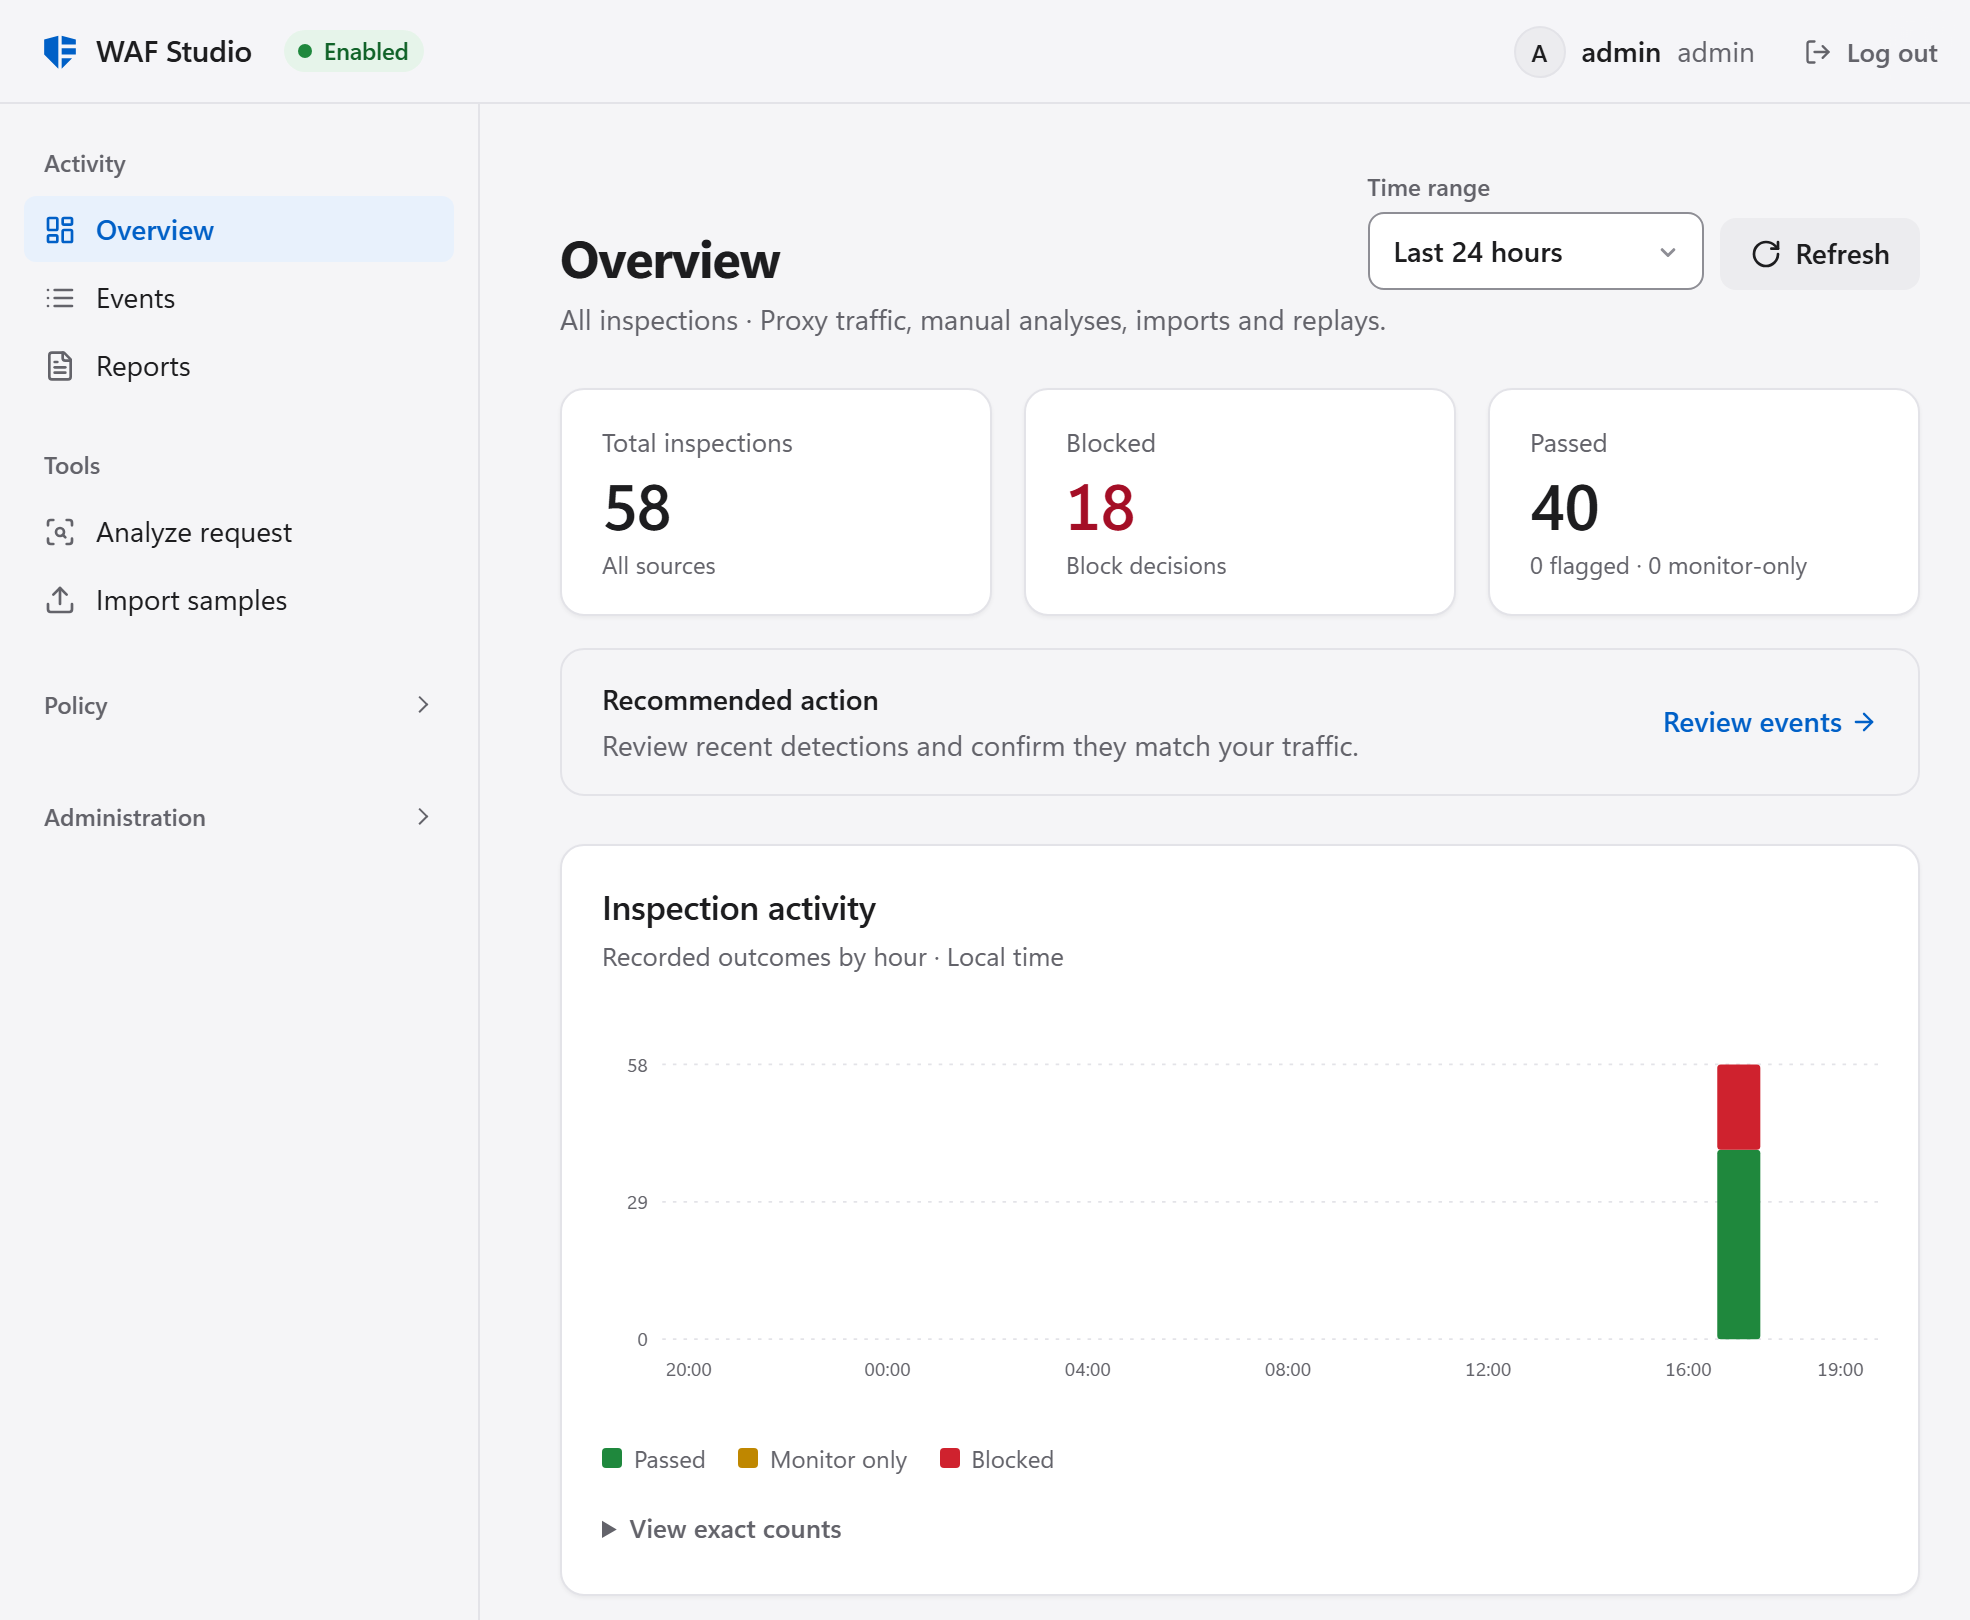
\includegraphics[width=0.7\textwidth]{Figures/dashboard.png}
\caption{The Overview screen: outcome cards, recommended action and hourly activity.}
\label{fig:dash}
\end{figure}

\section{Explainable Evidence}
Opening an event shows the evidence behind the decision across three focused cards (\emph{Decision \& score}, \emph{Rule matches} and \emph{Request \& metadata}): the unified outcome badge, each matched rule with its points and location, the total score against the thresholds, any parser anomalies or rate-limit state, and a recommendation that explains how to request a scoped exception instead of disabling a rule (Figure~\ref{fig:evidence}).

\begin{figure}[!h]
\centering
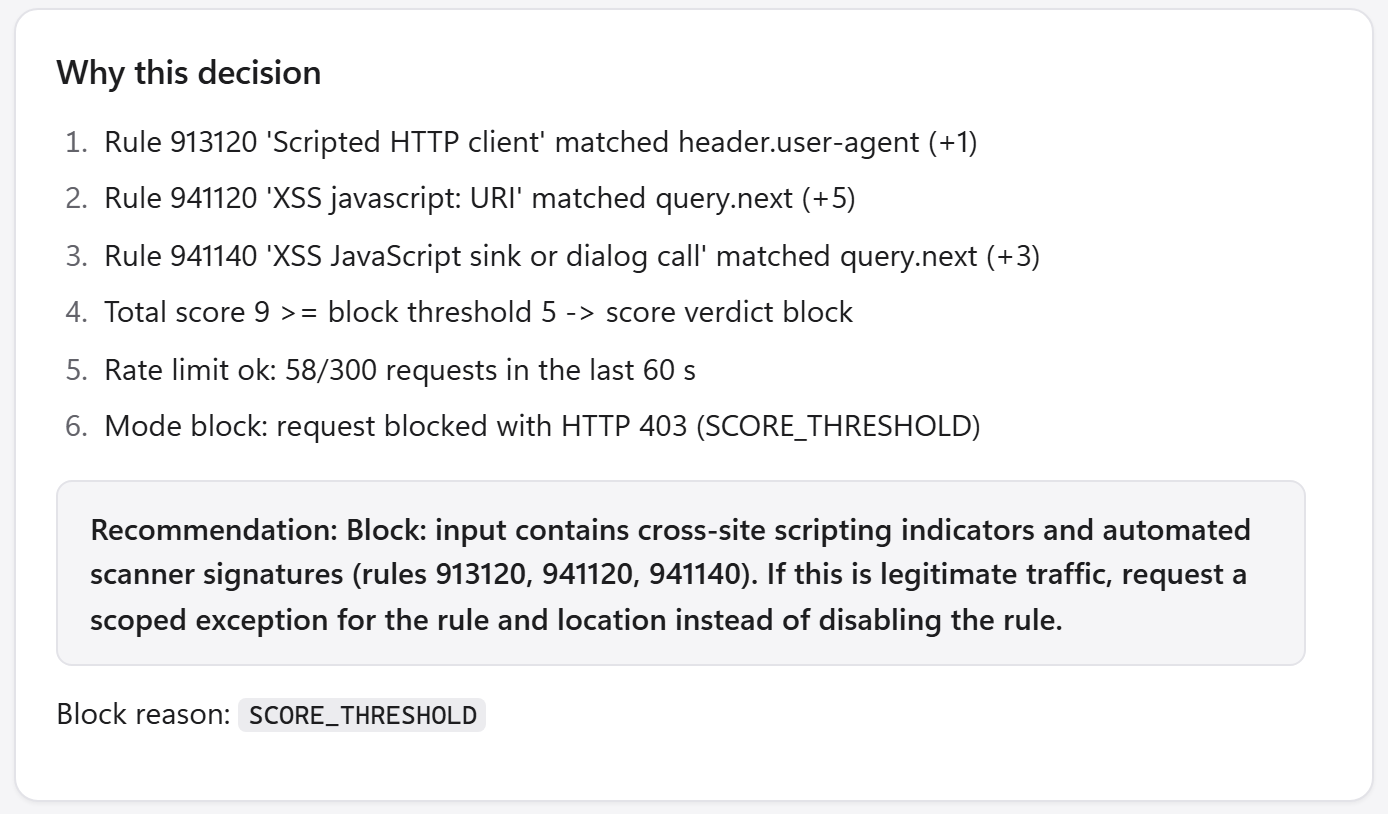
\includegraphics[width=0.85\textwidth]{Figures/evidence.png}
\caption{Decision explanation and recommendation for a blocked request with a score of 9.}
\label{fig:evidence}
\end{figure}

\section{Reports and Audit Log}
Events can be exported as JSON, CSV or HTML. Exports contain redacted excerpts of at most 120 characters and never secret headers, cookies, passwords or session data; HTML output is escaped and CSV cells are protected against spreadsheet formula injection. Every security-relevant action is written to an append-only audit log in which each record stores the hash of the previous one. Database triggers reject updates and deletes, and the Verify chain button reports ``Hash chain verified'' or the first broken link.

\section{Security of the Application}
Because the console displays attack payloads as evidence, its own security was treated as a requirement (Table~\ref{tab:controls}). The STRIDE threat model covers five trust boundaries and 13 data flows and maps 20 threats to mitigations, code and tests.

\begin{table}[!h]
\centering
\caption{Main security controls and what each one prevents.}
{\small\singlespacing\renewcommand{\arraystretch}{1.3}
\begin{tabular}{|p{6.0cm}|p{7.5cm}|}
\hline
\textbf{Control} & \textbf{What it prevents} \\
\hline
Server-enforced roles & A viewer reaching admin actions \\
\hline
scrypt hashes, hashed session tokens, CSRF binding, 30-minute idle and 8-hour absolute expiry & Stolen database contents, session reuse and forged requests \\
\hline
Parameterized SQL, strict input schemas & Injection into the application's own database \\
\hline
Text-only DOM construction and strict CSP & Attack samples running inside the console \\
\hline
Redaction and HMAC client pseudonyms & Secrets and raw IP addresses in stored evidence \\
\hline
Append-only, hash-chained audit log & Unnoticed edits to the record \\
\hline
\end{tabular}}
\label{tab:controls}
\end{table}

%==================================================================
\chapter{Evaluation}
\section{Method}
The evaluation starts the full stack on ephemeral localhost ports with a new temporary database, sends fixture requests through the real proxy to the vulnerable shop, and reads each stored event back through the API. It records the input, the expected and actual result, the matched rules, the score and the explanation. It ran on Node v24.19.0 under Windows on an Intel Core Ultra 7 255H with 16 logical processors, with engine version 1.0.0, 41 rules and the default thresholds. Expectations were set as protection goals before measurement; missed evasions remain expected to block and are reported as failures.

\section{Automated Acceptance and Mandatory Cases}
The strict acceptance run passed 782 of 782 tests in 36 suites, with no skipped tests and no vulnerabilities reported for the production dependencies. The mandatory evaluation passed 117 of 123 checks (95.1\%) as shown in Table~\ref{tab:cases}. These regression tests are separate from the evaluation, and passing them does not mean every attempted bypass was blocked.

\begin{table}[!h]
\centering
\caption{Mandatory evaluation cases and results.}
{\small\singlespacing\renewcommand{\arraystretch}{1.3}
\begin{tabular}{|p{6.2cm}|p{2.6cm}|p{4.5cm}|}
\hline
\textbf{Case} & \textbf{Passed} & \textbf{Note} \\
\hline
Injection strings (SQLi, XSS, traversal) & 28 of 28 & All blocked \\
\hline
Encoding and normalization variants & 20 of 20 & All blocked \\
\hline
Difficult benign inputs & 38 of 38 & All allowed \\
\hline
Large bodies and size limits & 6 of 6 & Window blind spot observed \\
\hline
Evasion attempts & 12 of 18 & Six misses kept as failures \\
\hline
Latency overhead & 2 of 2 & Below 25 ms \\
\hline
Failure, denial and restart & 11 of 11 & Safe behaviour, state persisted \\
\hline
\textbf{Total} & \textbf{117 of 123} & \textbf{95.1\%} \\
\hline
\end{tabular}}
\label{tab:cases}
\end{table}

\section{Detection Corpus}
A separate controlled corpus of 80 attack requests and 68 benign requests gave 76 true positives, 4 false negatives, 68 true negatives and no false positives (Table~\ref{tab:corpus}). Figure~\ref{fig:cov} shows coverage by category. The four misses are SQL split across parameters or JSON fields, base64-wrapped markup and a hexadecimal comparison, all of which need the application to reassemble the payload.

\begin{table}[!h]
\centering
\caption{Detection metrics on the controlled corpus.}
{\small\singlespacing\renewcommand{\arraystretch}{1.3}
\begin{tabular}{|p{6.4cm}|p{4.6cm}|}
\hline
\textbf{Metric} & \textbf{Value} \\
\hline
TP / FN / TN / FP & 76 / 4 / 68 / 0 \\
\hline
Precision & 100\% \\
\hline
Recall & 95\% \\
\hline
F1 score & 0.974 \\
\hline
Engine decision time (p50 / p95 / p99) & 0.234 / 0.476 / 0.776 ms \\
\hline
\end{tabular}}
\label{tab:corpus}
\end{table}

\begin{figure}[!h]
\centering
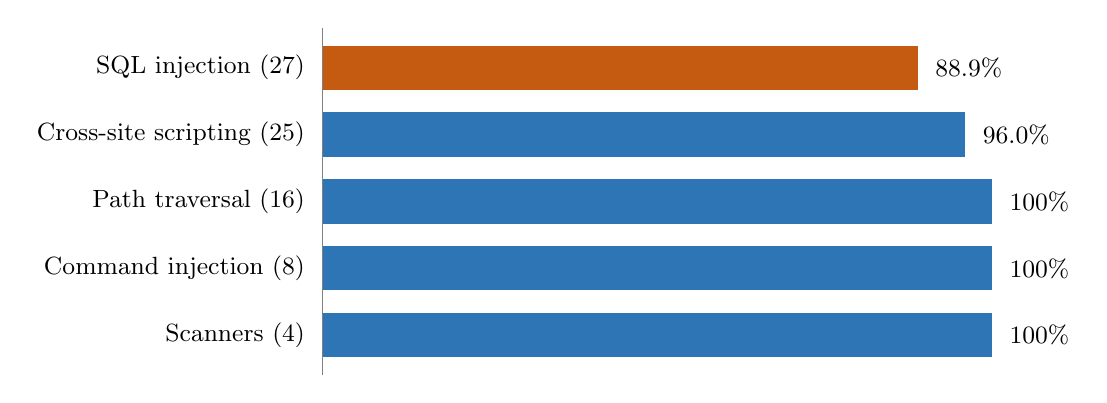
\begin{tikzpicture}[font=\small]
  \foreach \i/\n/\v/\c in {0/{SQL injection (27)}/88.9/worange, 1/{Cross-site scripting (25)}/96.0/wblue, 2/{Path traversal (16)}/100/wblue, 3/{Command injection (8)}/100/wblue, 4/{Scanners (4)}/100/wblue} {
    \pgfmathsetmacro{\y}{-\i*0.85}
    \pgfmathsetmacro{\w}{\v*0.085}
    \node[anchor=east] at (0,\y) {\n};
    \fill[\c] (0.1,\y-0.28) rectangle (0.1+\w,\y+0.28);
    \node[anchor=west] at (0.2+\w,\y) {\v\%};
  }
  \draw[gray] (0.1,0.5) -- (0.1,-3.9);
\end{tikzpicture}
\caption{Detection coverage by attack category (attack samples in brackets).}
\label{fig:cov}
\end{figure}

\section{Latency Overhead}
The benchmark used 300 interleaved request pairs per scenario after 30 warm-up requests. Proxy timing includes inspection, event storage and forwarding. The added time at the 95th percentile was below 2 ms for both scenarios, well under the 25 ms teaching-tool target (Table~\ref{tab:latency}), and no request failed.

\begin{table}[!h]
\centering
\caption{Response time at the 95th percentile, in milliseconds.}
{\small\singlespacing\renewcommand{\arraystretch}{1.3}
\begin{tabular}{|p{4.2cm}|p{2.4cm}|p{2.9cm}|p{2.4cm}|}
\hline
\textbf{Scenario} & \textbf{Direct} & \textbf{Through WAF} & \textbf{Added} \\
\hline
GET search & 0.378 & 2.266 & 1.888 \\
\hline
POST 2 KiB form & 0.337 & 2.325 & 1.988 \\
\hline
\end{tabular}}
\label{tab:latency}
\end{table}

%==================================================================
\chapter{Limitations and Conclusion}
\section{Known Limitations}
The six missed evasion attempts are SQL tokens split across parameters or JSON fields, base64-wrapped markup, a hexadecimal numeric comparison, a string-concatenated comparison, and markup split across duplicate parameters. Per-value matching cannot rebuild payloads that only the application joins together.

Other boundaries are the 64~KiB body inspection window, a heuristic regular-expression guard, rate-limit windows kept in memory, no inspection of responses, no TLS on the loopback interface, pattern-based secret redaction, and an audit chain that is not anchored outside the database, so it detects ordinary tampering but cannot stop someone who rewrites the whole file. The test shop is reachable by other local processes.

The evaluation results come from a small synthetic corpus that shares signature families with the other tests, run on one laptop. They show how the engine behaves in the lab and must not be generalized to internet traffic.

\section{Conclusion}
WAF Studio meets the proposal's objectives: it makes explainable decisions through both a reverse proxy and a console, supports safe tuning with two-person approval of exceptions, keeps tamper-evident evidence, and protects its own users and data. Its measured behaviour and its limits are both reported openly.

Future work could add response inspection, anchoring of the audit chain outside the database, TLS termination, cross-parameter reconstruction for split payloads, and an independent test corpus.

\end{document}
